\documentclass[a4paper]{article}

% Essentials
\usepackage[utf8]{inputenc}
\usepackage[english]{babel}
\usepackage{hyperref}
\usepackage[table]{xcolor}

% Hyperlinks
\hypersetup{
    colorlinks,
    linkcolor={red},
    citecolor={blue},
    urlcolor={blue}
}

% Optional but very useful
\usepackage[tmargin=3.5cm, bmargin=3.5cm, lmargin=3cm, rmargin=3cm]{geometry}
\usepackage{amsmath,amsthm,amsfonts,amssymb}
\usepackage{graphicx}
\usepackage{multicol}
\usepackage{float}
\usepackage{enumitem}
\usepackage{tabularx,booktabs,multirow}
\usepackage{longtable}
\usepackage{url}
\usepackage{enumitem}
\usepackage{todonotes}
\usepackage{caption}

% \sam comment command
\newcommand{\sam}[1]{{\color{red}(#1)}}

% \range* commands
\newcommand{\range}[3]{#1[#2,#3]}
\newcommand{\rangeto}[2]{#1{:}#2}
\newcommand{\rangeall}{:}

% Title
\title{Excel Constraints}
\date{\today}

% Indentation
\setlength\parindent{0pt}

\begin{document}

\maketitle

% Content

\section{Use cases} % (fold)
\label{sec:use_cases}
There are different ways that learned constraints could be used in practice:

\begin{itemize}
	\item Find mistakes
	\item Suggest a formula for a specific field
	\item Suggest a next value / autosuggest
	\item Find structure and functions in a plain text sheet (such as a csv)
\end{itemize}

% section use_cases (end)

\section{Desired output} % (fold)
\label{sec:demo_example}
The annotated example (fig.~\ref{fig:demo}) demonstrates the most used constraints in Excel which we aim to identify automatically.

% section demo_example (end)
\begin{description}
	\item[Aggregates] Aggregate functions like sum, max, average, ... that reduce a range to a value
	\item[Conditional aggregates] Aggregates that use a filter on their input
	\item[Series] Ranges of integer numbers, ascending or descending (a special case of a permutation)
	\item[Lookups] Exact or fuzzy lookups that use a key to find a corresponding value
	\item[Ranks] Uses a range and a value to determine an order over elements
	\item[Structural constraints] Foreign keys to test value consistency between ranges
	\item[Previous] Uses row values and the previous value to compute the current value
\end{description}

Notable omission so far is the \textit{if-then-else} constraint. Whether it will be included and if how this will be done exactly is still to be determined.

Generally these constraints can be subdivided into:

\begin{itemize}
	\item Row constraints
	\item Column constraints
	\item Inter-table constraints
	\item Nested constraints
\end{itemize}

\begin{figure}
  \centering
    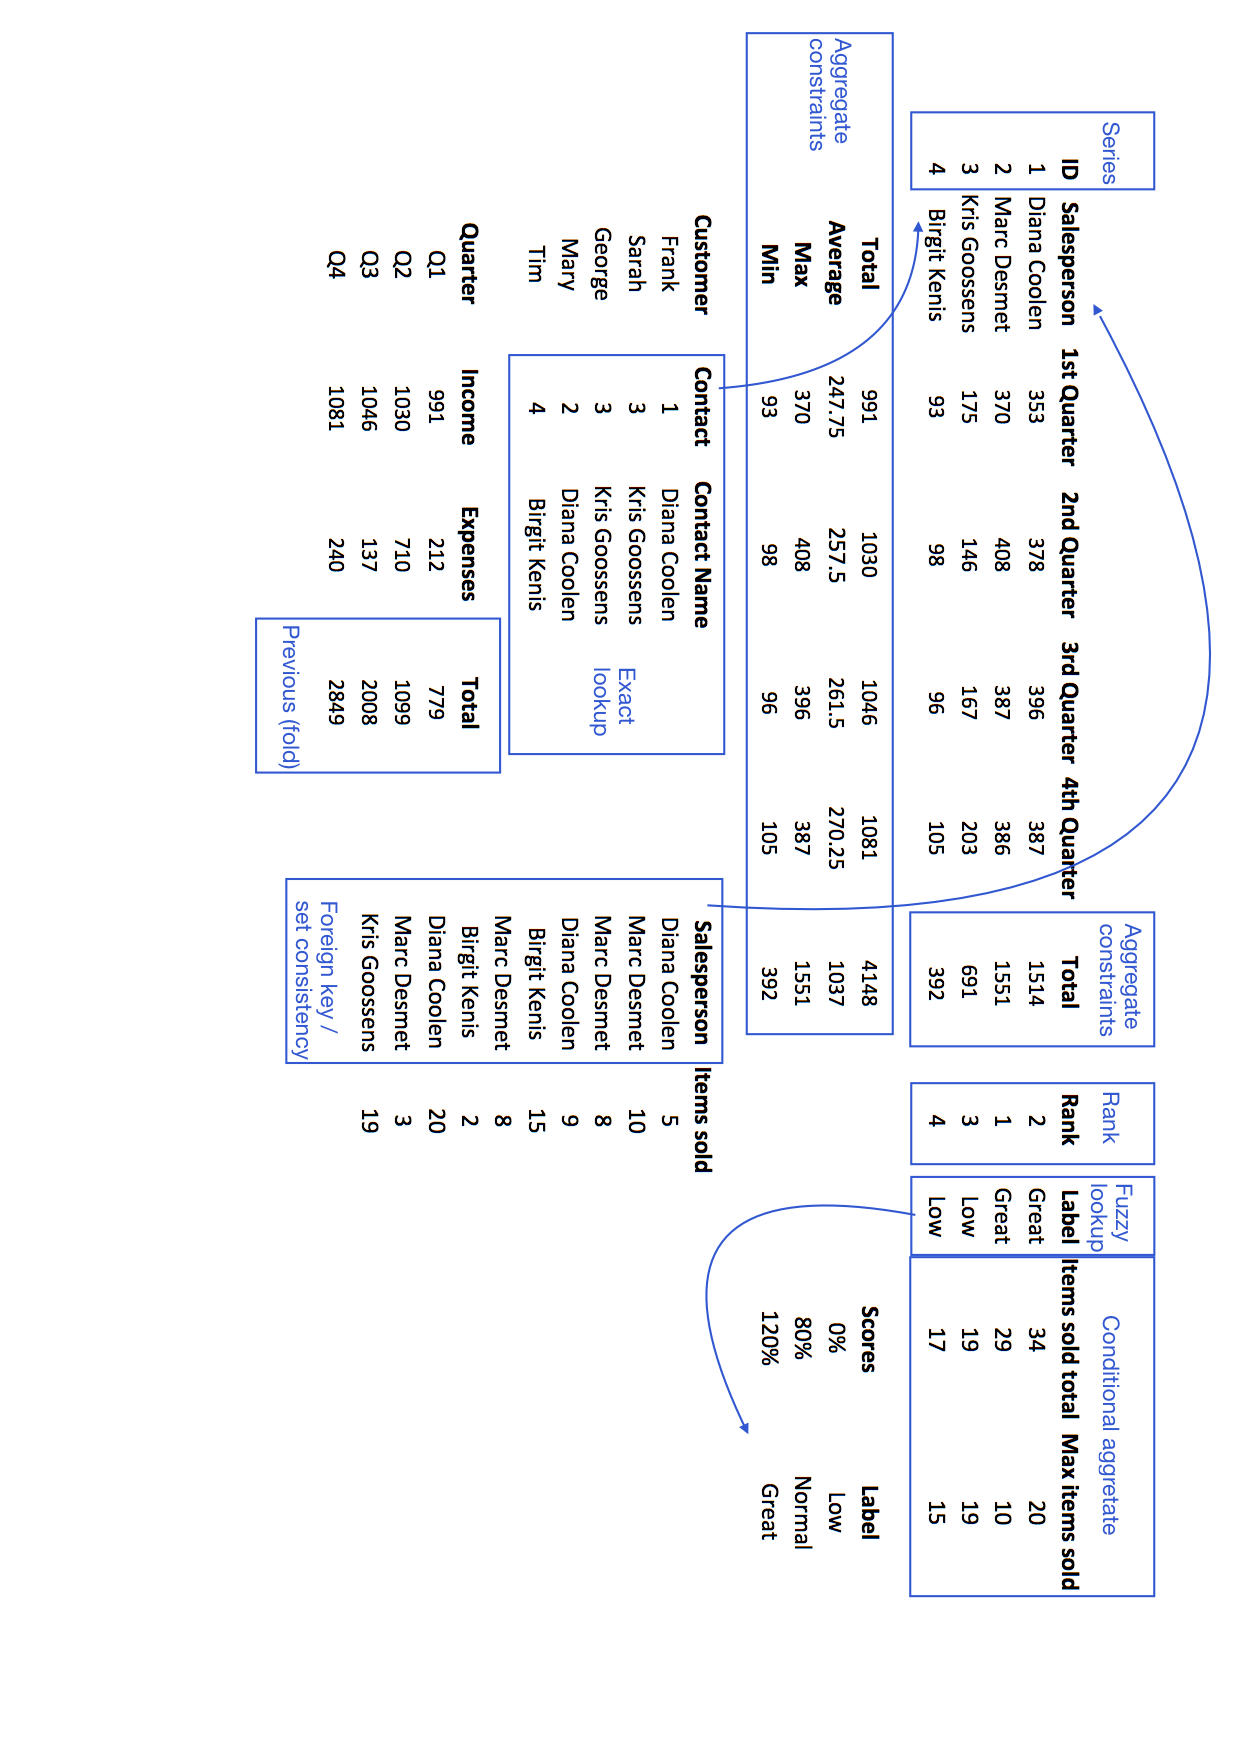
\includegraphics[width=1\linewidth]{../Demo.png}
  \caption{Demo example}
  \label{fig:demo}
\end{figure}

% section types_of_constraints (end)

\section{Approach} % (fold)
\label{sec:approach}

Currently we are considering a ModelSeeker like approach were ranges and values are generated and constraints tested upon them.
One option would be to use constraint-specific generators to avoid the explosion of the search space.
Meta-information would be used to find the most specific constraints.
A heuristic could use various information to determine which learned constraints are useful.

\subsection{Group discovery}
Vectors consist of columns or rows that are consistent in their type (e.g. the Salesperson column or the Average row).
Groups are sets of vectors that are consistent in their type and size.
If only neighboring vectors are allowed to be added to a group, the group consists of a range.
The groups partition the data and for every group subgroups may be defined that can overlap.

Groups describe subsets of data and can be used to form an $m \times n$ matrix with a specific type.
Constraints can then be defined in terms of these matrices.

Our current approach would be to precompute all groups and subgroups and store metadata about their content (e.g. type, size) and hierarchy (e.g. child and parent groups).

An important consideration is that some data could be considered input while other data might have to be computed.
This influences the search algorithm.

\subsection{Finding constraints}
Currently we see three approaches to finding constraints:

\begin{description}
	\item[Constraint view] In this approach the search for constraints is structured foremost from the point of view of the constraints.
	This means that for every type of constraint groups and transformations  are searched such that they fulfill the constraint.
	\item[Vector view] From an Excel point of view constraints are typically functional.
	Constraint are either a property of a vector (e.g. series) or describe how a specific vector can be calculated in terms of other vectors (e.g. sum).
	This lead us to the vector view in which for every vector constraints are searched that hold on the vector or describe how to calculate it.
	\item[Set view] The last approach is to generate sets of groups and test various constraints on the set.
	This approach seems simpler but also more naive than the previous approaches.
\end{description}

In order to choose what groups may occur in what constraints and what combinations are valid, metadata about the constraints is also required (e.g. consistency in sizes, types).
Additionally the system needs information about the relation between different constraints to remove redundancies.

\subsection{Transformations}
So far the concept of transformations is only defined losely.
The idea is that some constraints cannot act on groups without applying a transformation on one or multiple groups first (e.g. the \textit{previous} transformation).
Therefore, there should be a catalog of transformations which might be applied to groups.
As with constraints, metadata about the transformations should be given.
It is yet a bit unclear what the difference is between transformations and constraints.
On one hand, one might see some constraints as transformations and vice versa.
One could generalize to \textit{functions} that map input to output.
On the other hand, however, a property of transformations could be that they preserve their input size and distantiate them from constraint / functions in that way.
Considering transformations separately might avoid some of the combinatorial explosion that arbitrary function chaining might provide.

One notable decision about transformations in general will be if the system supports types of backwards reasoning.
An easy example of this would be adding a constant to the input or multiplying it with a constant.

\section{Notation}
\subsection{Ranges}
Every table $T$ is considered like a matrix.
Indexing allows to specify a subset of the table, for example, $\range{T}{r}{c}$ represents the cell at row~$r$ and column~$c$.
The colon $:$ is used to represent ranges.
For example, $\range{T}{\rangeall}{c}$ selects all cells in column~$c$ and $\range{T}{\rangeto{r_1}{r_2}}{\rangeall}$ selects all cells in the rows $r_1$ to $r_2$.
Disjoint columns can be specified by using $\range{T}{\rangeall}{\{c_1, ..., c_n\}}$.

\subsection{Example}
\paragraph{Aggregates}
There are two types of aggregates in the example: The \textit{Total} column consists of the sum of the four previous columns and the \textit{Total} row consist of the sum of the column corresponding to each cell.
These constraints can be written as:
\begin{align}
	\range{T_1}{\rangeall}{7} = \mathit{SUM}(\range{T_1}{\rangeall}{\rangeto{3}{6}}, row)\\
	\range{T_2}{\rangeall}{1} = \mathit{SUM}(\range{T_1}{\rangeall}{\rangeto{3}{7}}, column).
\end{align}

\paragraph{Conditional aggregates}
Conditional aggregates form more challenging constraints.
There is an arbitrary reduction in size of the input data based on a condition to be matched.
The complexity of this constraint is also dependent on the restrictions imposed on the constraint part.
The conditional sum that calculates the \textit{Items sold total} column uses exact matching the salesperson name. Sticking close to the Excel notation this could be written as:
\begin{align}
	\range{T_1}{\rangeall}{10} = \mathit{SUMIF}(\range{T_5}{\rangeall}{1}, \range{T_1}{\rangeall}{2}, \range{T_5}{\rangeall}{2}).
\end{align}
Here, the condition will be applied to the \textit{Salesperson} column of table~5 (the test vector).
Generally speaking the test vector has to match the sum column in size and the condition vector has to match the output vector.
However, the condition can also consist of a boolean test such as $>5$ or a single value.
To represent these constraints the Excel style using strings or exact values could be used but this might change yet to accomodate possibly more expressive conditions.

\paragraph{Unary}
The \textit{ID} column consists of a series:
\begin{align}
	\mathit{SERIES}(\range{T_1}{\rangeall}{1}).
\end{align}
Series are general cases of permutations.
If a vector of size $n$ is a permutation of the numbers $[1, n]$, this can be an interesting observation, but often it is an interesting property of the vector which might unlock other constraints.
See, for example, the column \textit{Rank} which is a permutation ($\mathit{PERMUTATION}(\range{T_1}{\rangeall}{8})$).
This property allows the rank constraint to be applied to it (See below).
Similarly, all-different constraints can be uselful as constraint or precondition.
For numberic data all-different is not very useful but it might be for textual data such as colum \textit{Salesperson} ($\mathit{ALLDIFFERENT}(\range{T_1}{\rangeall}{2})$).
Here, the all-different property allows the column to be refered to by a foreign key.

\paragraph{Lookups}
Consider the exact lookup in the example.
This constraint can be expressed as:
\begin{align}
	\range{T_4}{\rangeall}{3} = \mathit{LOOKUP}(\range{T_1}{\rangeall}{1}, \range{T_1}{\rangeall}{2}, \range{T_4}{\rangeall}{2}).
\end{align}
Lookups, however, also support more complex constraints.
For example, a fuzzy lookup assigns values to intervals to lookup the output value.
Moreover, the input values can be transformed.
The fuzzy lookup for the \textit{Label} column demonstrates this:
\begin{align}
	\range{T_1}{\rangeall}{9} = \mathit{LOOKUP}(\range{T_1}{\rangeall}{7} / \range{T_2}{2}{5}, \range{T_3}{\rangeall}{1}, \range{T_3}{\rangeall}{2}).
\end{align}
Here, the \textit{Total} column is divided by the calculated total average before being used to lookup what interval the performance falls into.

\paragraph{Ranks}
The column \textit{Rank} ranks based on the the column \textit{Total}, which can be expressed as:
\begin{align}
	\range{T_1}{\rangeall}{8} = RANK(\range{T_1}{\rangeall}{7}).
\end{align}

\paragraph{Structural constraints}
The \textit{Salesperson} column in table~5 can be seen as a foreign key refering to the corresponding column in table~1.
There are different options of representing this constraint:
\begin{align}
	\mathit{UNIQUE}(\range{T_5}{\rangeall}{1}) \subseteq \range{T_1}{\rangeall}{2} \label{eq:unique}\\
	\mathit{FOREIGNKEY}(\range{T_1}{\rangeall}{2}, \range{T_5}{\rangeall}{1}) \label{eq:foreign_key}
\end{align}
Equation~\ref{eq:unique} uses a size-changing transformation or non-reversible function to express the underlying property.
Instead one could also introduce a binary constraint expressing the foreign-key property directly (as in equation~\ref{eq:foreign_key}).

\paragraph{Previous} Using the previous value in the constraint for a field can be solved easily by using a transformation.
The calculation of the \textit{Total} column of table $T_6$ can be expressed as:
\begin{align}
	\range{T_6}{\rangeall}{4} = \range{T_6}{\rangeall}{2} - \range{T_6}{\rangeall}{3} + \mathit{PREVIOUS}(0, \range{T_6}{\rangeall}{4}, column).
\end{align}
The previous transformation drops the last value and adds an initial value, maintaining the size of the transformation input.
In this specific case it is worth noting that this constraint can also be expressed differently:
\begin{align}
	\range{T_6}{\rangeall}{2} = \mathit{SUM}(\range{T_6}{\rangeall}{\rangeto{3}{4}}, row).
\end{align}
This constraint makes a different assumption about which columns are considered input and which are considered output.
If no additional information is given, the algorithm could decide to provide both (redundant) constraints, or make a decision based on generality / specificity or a heuristic.

\end{document}